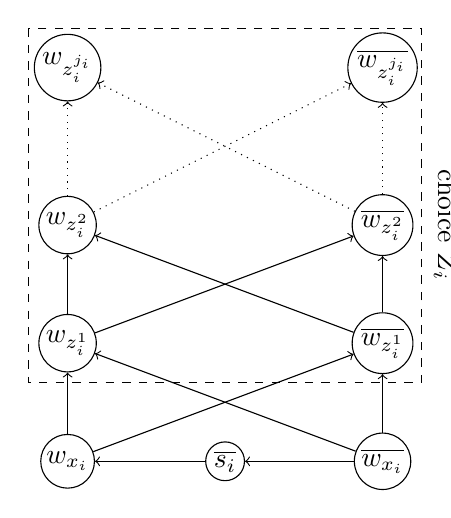
\begin{tikzpicture}[every node/.style={circle, draw, inner sep=1pt}]

\node (v3) at (-2,0.5) {$w_{x_i}$};
\node (v2) at (0,0.5) {$\overline{s_i}$};
\node (v1) at (2,0.5) {$\overline{w_{x_i}}$};
\draw [->] (v1) edge (v2);
\draw [->] (v2) edge (v3);
\draw [dashed] (-2.5,6) rectangle (2.5,1.5);

\draw [use as bounding box,draw=none] (-2.5,6) rectangle (2.5,0.2);

\node (v4) at (-2,2) {$w_{z_i^1}$};
\node (v6) at (2,2) {$\overline{w_{z_i^1}}$};
\node (v5) at (-2,3.5) {$w_{z_i^2}$};
\node (v7) at (2,3.5) {$\overline{w_{z_i^2}}$};
\node (v8) at (-2,5.5) {$w_{z_i^{j_i}}$};
\node (v9) at (2,5.5) {$\overline{w_{z_i^{j_i}}}$};
\draw [->] (v4) edge (v5);
\draw [->] (v6) edge (v7);
\draw [->] (v4) edge (v7);
\draw [->] (v6) edge (v5);

\draw [->,dotted] (v5) edge (v8);
\draw [->,dotted] (v7) edge (v9);
\draw [->,dotted] (v7) edge (v8);
\draw [->,dotted] (v5) edge (v9);
\draw [->] (v3) edge (v4);
\draw [->] (v3) edge (v6);
\draw [->] (v1) edge (v4);
\draw [->] (v1) edge (v6);

\node [draw=none,rotate=-90] (ch) at (2.8,3.5) {choice $Z_i$};
\end{tikzpicture}